\documentclass[tikz,border=8pt]{standalone}
% Shared look for every TikZ diagram. Load with \input{../../tools/tikz-style.tex}
\usepackage[T1]{fontenc}
\usepackage{lmodern}
\renewcommand{\sfdefault}{lmr}  % diagrams use the same serif as the text
\usetikzlibrary{arrows.meta, positioning, shapes.geometric, calc, fit, backgrounds}
\definecolor{cblue}{HTML}{4C78A8}
\definecolor{corange}{HTML}{F58518}
\definecolor{cgreen}{HTML}{54A24B}
\definecolor{cred}{HTML}{E45756}
\definecolor{cpurple}{HTML}{B279A2}
\definecolor{cgrey}{HTML}{6B6B6B}
\tikzset{
  every picture/.style={font=\sffamily, line width=1.2pt},
  box/.style={draw=#1, fill=#1!12, rounded corners=4pt, align=center, inner sep=7pt, minimum height=1.1cm},
  box/.default=cgrey,
  arrow/.style={-{Stealth[length=3mm]}, draw=cgrey, line width=1.4pt},
  title/.style={font=\sffamily\bfseries\Large},
  note/.style={font=\sffamily\small, text=cgrey, align=center},
}
\AtBeginDocument{\hyphenpenalty=10000 \exhyphenpenalty=10000}

% Velocity model, noise-free: v = 0.5 m/s, omega = 1 rad/s, so R = v/omega = 0.5 m. The turning point C lies R to the
% robot's left, at (1.75, 1.433). In 1 s the robot turns 1 rad about C and ends at (2.249, 1.409), heading 87.3 deg.
\begin{document}
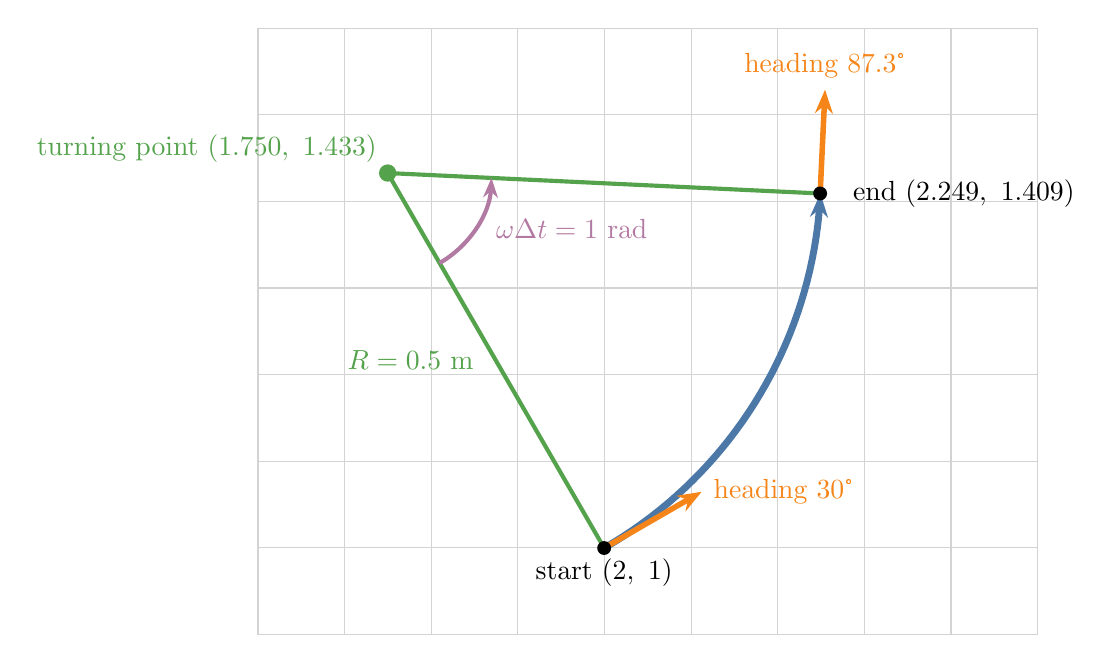
\begin{tikzpicture}[scale=11, every node/.append style={font=\large}]
  \coordinate (A) at (2,1); \coordinate (C) at (1.75,1.433); \coordinate (B) at (2.2494,1.4094);
  \draw[cgrey!30, line width=0.4pt] (1.6,0.9) grid[step=0.1] (2.5,1.6);
  \draw[cblue, line width=2.5pt, -{Stealth[length=3mm]}] plot[domain=0.5236:1.5236, samples=40] ({1.75+0.5*sin(\x r)}, {1.433-0.5*cos(\x r)});
  \draw[cgreen, line width=1.5pt] (A) -- (C) node[midway, left=4pt, font=\normalsize] {$R = 0.5$ m};
  \draw[cgreen, line width=1.5pt] (C) -- (B);
  \draw[cpurple, line width=1.5pt, -{Stealth[length=2.5mm]}] ($(C)+(-60:0.12)$) arc (-60:-2.7:0.12);
  \node[cpurple, right, font=\normalsize] at ($(C)+(-30:0.13)$) {$\omega\Delta t = 1$ rad};
  \draw[-{Stealth[length=3mm]}, corange, line width=2pt] (A) -- ++(30:0.13) node[right, font=\normalsize] {heading 30°};
  \draw[-{Stealth[length=3mm]}, corange, line width=2pt] (B) -- ++(87.3:0.12) node[above, font=\normalsize] {heading 87.3°};
  \fill[black] (A) circle (0.008) node[below, font=\normalsize] {start $(2,\ 1)$};
  \fill[cgreen] (C) circle (0.01) node[above left, font=\normalsize] {turning point $(1.750,\ 1.433)$};
  \fill[black] (B) circle (0.008) node[right=8pt, font=\normalsize] {end $(2.249,\ 1.409)$};
\end{tikzpicture}
\end{document}
